% !TEX TS-program = pdflatex
% !TeX program = pdflatex
% !TEX encoding = UTF-8
% !TEX spellcheck = fr

\documentclass[12pt, a4paper]{article}
%\usepackage{fullpage}
\usepackage[left=2cm,right=1.5cm,top=1.5cm,bottom=1.5cm]{geometry}
\usepackage[fleqn]{amsmath}
\usepackage{amssymb,wasysym}

\usepackage[T1]{fontenc}
\usepackage[utf8]{inputenc}
\usepackage[french,english]{babel}
\usepackage{txfonts} 
\usepackage[]{graphicx}
\usepackage{multirow}
\usepackage{hyperref}
\usepackage{parskip}
\usepackage{turnstile}%Induction symbole
\usepackage{enumitem}
\usepackage{color}


\renewcommand{\baselinestretch}{1}

\newcommand{\ou}{\ |\ }

\begin{document}

\selectlanguage {french}
%\pagestyle{empty} 

\noindent\rule{\textwidth}{1pt}\\[0.25cm]
\noindent
\begin{tabular}{ll}
\multirow{3}{*}{
\includegraphics[width=2.5cm]{....//extra/logo/esi-logo.png}} & \'Ecole national Supérieure d'Informatique\\
& 2\textsuperscript{ième} année cycle supérieur (2023-2024)\\
& Système intelligents et données (SID)\\
& Machine Learning\\
\end{tabular}\\[.25cm]
\noindent
\begin{center}
{\LARGE\bfseries Workshop 02. Données, algorithmes et ensembles}\\
\end{center}
\noindent\rule{\textwidth}{1pt}

%Ce TP n'est pas noté.
%Cependant, vous devez rendre une portion à la fin de la séance.

\section{Données}

Dans cette section, nous voulons apprendre quelques traitements sur les données.

\subsection{Lecture des données}

\begin{itemize}
	\item Télécharger le dataset satellite\footnote{\url{https://archive.ics.uci.edu/ml/datasets/Statlog+(Landsat+Satellite)}}.
	\item Importer les données d'entraînement (sat.trn) et de test (sat.tst).
	\item Diviser les en X\_train, Y\_train, X\_test et Y\_test.
\end{itemize}

\subsection{Analyse des données}

\begin{itemize}
	\item Tracer le diagramme en boîte des 3 premières caractéristiques (train), figure \ref{res-analyse}(a).
	\item Tracer le graphique en secteurs du tailles des classes (train), figure \ref{res-analyse}(b).
	\item Appliquer l'ACP (2 composantes) de scikit-learn sur le dataset d'entrainement.
	\item Tracer le nuage des échantillons selon ces deux composantes (train), figure \ref{res-analyse}(c).
	\item Tracer le nuage des échantillons selon ces deux composantes (test), figure \ref{res-analyse}(d).
	\item Discuter les résultats.
	\begin{itemize}
		\item Variance des caractéristiques.
		\item Distribution des classes.
		\item Distribution des échantillons selon ACP.
	\end{itemize}
\end{itemize}

\begin{figure}[ht]
	\centering
	\begin{tabular}{cccc}
		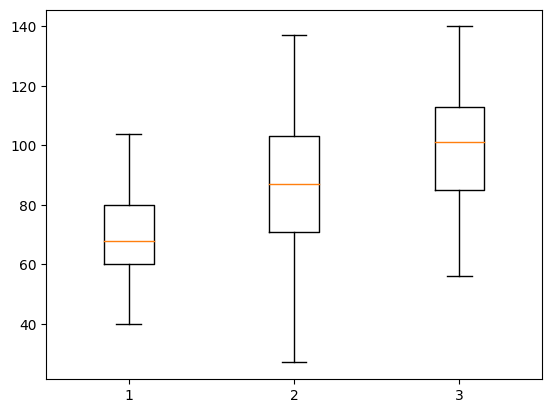
\includegraphics[width=0.22\textwidth]{../img/workshop/stat.png} &
		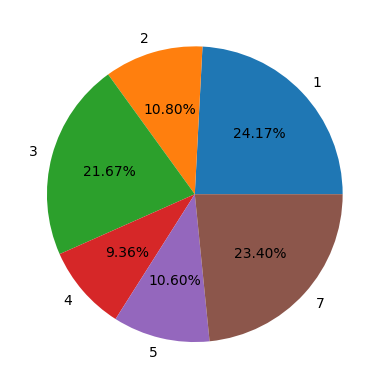
\includegraphics[width=0.22\textwidth]{../img/workshop/cls.png} &
		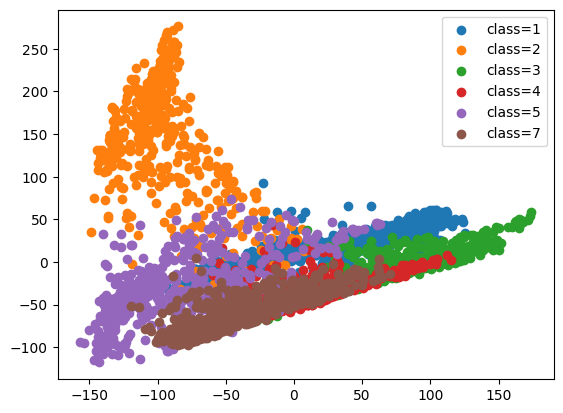
\includegraphics[width=0.22\textwidth]{../img/workshop/pca.train.png} &
		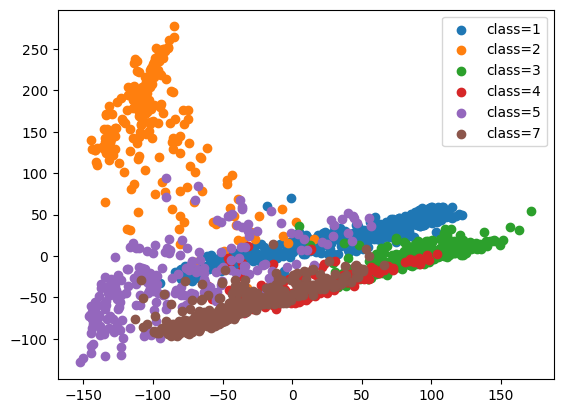
\includegraphics[width=0.22\textwidth]{../img/workshop/pca.test.png} \\
		(a) Statistiques &
		(b) \% classes  &
		(c) ACP entrainement &
		(d) ACP test \\
	\end{tabular}
	\caption{Résultats d'analyse}
	\label{res-analyse}
\end{figure}

\subsection{Échantillonnage des données}

\begin{itemize}
	\item Installer l'outil \textbf{imblearn}.
	\item Appliquer deux sous-echantillonages : ClusterCentroids et TomekLinks sur X\_train.
	\item Appliquer le sur-echantillonages SMOTE sur X\_train.
	\item Entrainer 4 modèles de régression logistique avec régularisation L2 (par défaut) avec le solveur ``liblinear" sur les données originales, sous-échantillonnées et sur-échantillonnées.
	\item Comparer l'exactitude (accuracy) pour ces modèles dans l'entrainement et le test.
\end{itemize}

\begin{center}
	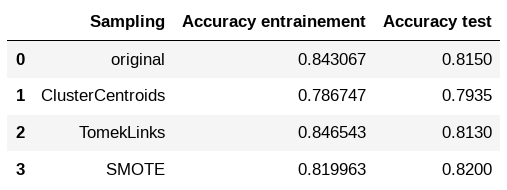
\includegraphics[width=0.5\textwidth]{../img/workshop/sampling.png}
\end{center}

\section{Algorithmes}

Dans cette section, nous voulons comparer des algorithmes de classement en se basant sur quelques critères.

\subsection{Entraînement et test}

\begin{itemize}
	\item Entraîner les modèles suivants : Régression logistique avec régularisation L2 (par défaut) et le solveur ``liblinear", Naïve Bayes Gaussien, Arbre de décision CART et Forêt aléatoire avec 50 estimateurs (arbres).
%	\begin{itemize}
%		\item Régression logistique avec régularisation L2 (par défaut) et le solveur ``liblinear"
%		\item Naïve Bayes Gaussien 
%		\item Arbre de décision CART
%		\item Forêt aléatoire avec 50 estimateurs (arbres)
%	\end{itemize}
	\item Pour chaque modèle, récupérer les informations suivantes : Temps d'entraînement, Temps de test, Exactitude (Accuracy) d'entraînement et Exactitude (Accuracy) de test.
%	\begin{itemize}
%		\item Temps d'entraînement
%		\item Temps de test
%		\item Exactitude (Accuracy) d'entraînement
%		\item Exactitude (Accuracy) de test
%	\end{itemize}
	\item Afficher un tableau qui résume ces critères
\end{itemize}

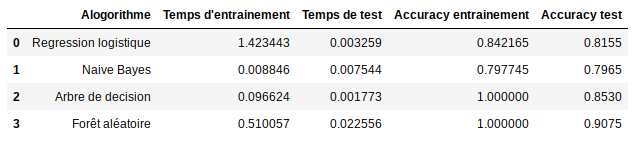
\includegraphics[width=\textwidth]{../img/workshop/criteres.png}

\subsection{Discussion}

\begin{itemize}
	\item En terme de temps d'entraînement
	\begin{itemize}
		\item Quel est l'ordre des algorithmes du plus rapide au plus lent ?
		\item Justifier ça en se basant sur la façon sur laquelle l'algorithme construit le modèle.
		\item Comment peut-on améliorer le temps d'entraînement de chaque algorithme (si on peut) ?
	\end{itemize}
	\item En terme de temps de test
	\begin{itemize}
		\item Quel est l'ordre des algorithmes du plus rapide au plus lent ?
		\item Justifier ça en se basant sur la façon sur laquelle le modèle estime la classe.
		\item Comment peut-on améliorer le temps d'estimation de chaque algorithme (si on peut) ?
	\end{itemize}
	\item En terme d'exactitude d'entraînement
	\begin{itemize}
		\item Quel est l'ordre des algorithmes du mieux convergé au pire ?
		\item Justifier ça en se basant sur la façon sur laquelle l'algorithme construit le modèle.
	\end{itemize}
	\item En terme d'exactitude de test
	\begin{itemize}
		\item Quel est l'ordre des algorithmes du mieux généralisé au pire ?
		\item Justifier ça en se basant sur la façon sur laquelle le modèle estime la classe.
	\end{itemize}
\end{itemize}

\section{Apprentissage ensembliste}

Ici, nous voulons comparer entre les algorithmes de classement (régression logistique, naïve Bayes et Arbre de décision) dans le contexte d'apprentissage ensembliste.
Les méthodes utilisées sont : 
\begin{itemize}
	\item Bagging ( Bootstrap aggregating) : Créer K Bootstraps (groupes aléatoires des échantillons). 
	Entraîner un modèle sur chaque Bootstrap.
	Lors d'estimation, un vote majoritaire sur les estimations des modèles est appliqué.
	\item Boosting : Entraîner un estimateur sur le dataset d'entraînement. 
	Appliquer des prédictions pour avoir les échantillons mal-estimés.
	Donner plus de poids à ces échantillons et entraîner un autre estimateur.
	Refaire la même chose jusqu'à avoir K estimateurs.
	Lors d'estimation, un vote majoritaire sur les estimations des modèles est appliqué.
	\item Stacking : Entraîner K estimateurs sur le même dataset d'entraînement.
	Ces estimateurs doivent avoir des hyper-paramètres différents ou des algorithmes d'apprentissage différents.
	Entraîner un estimateur qui a comme entrée les sorties des autres K estimateurs.
\end{itemize}

\subsection{Entraînement et test}

\begin{itemize}
	\item Entraîner les modèles suivants avec Bagging et Adaboost (10 estimateurs) : Régression logistique avec régularisation L2 (par défaut) avec le solveur ``liblinear", Naïve Bayes Gaussien et Arbre de décision CART.
%	\begin{itemize}
%		\item Régression logistique avec régularisation L2 (par défaut) avec le solveur ``liblinear"
%		\item Naïve Bayes Gaussien 
%		\item Arbre de décision CART
%	\end{itemize}
	\item Entraîner un modèle avec Stacking (l'estimateur de sortie est celui par défaut : régression logistique) avec les 3 algorithmes précédents.
	\item Afficher un tableau qui résume ces critères
\end{itemize}

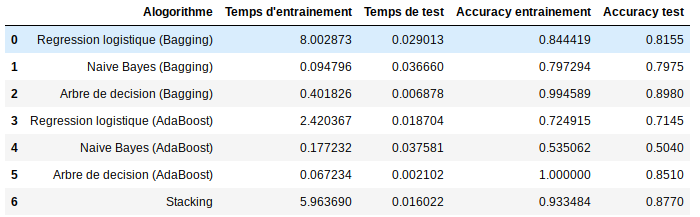
\includegraphics[width=\textwidth]{../img/workshop/criteres2.png}

\subsection{Discussion}

\begin{itemize}
	\item En terme de temps d'entraînement
	\begin{itemize}
		\item Pourquoi le temps d'entraînement du Bagging, en général, est plus grand que celui de AdaBoost ?
		\item Pourquoi le temps d'entraînement du Bagging est plus petit que celui d'AdaBoost en cas de Naïve Bayes ?
		\item Pouvons-nous améliorer ce temps en utilisant le parallélisme pour chaque méthode (Bagging, Boosting et Stacking) ?
		\item Si oui, décrire comment (supposant le nombre des machines est illimité) ? Si non, pourquoi ?
	\end{itemize}
	\item En terme de temps de test
	\begin{itemize}
		\item Pourquoi le temps de test du Bagging est similaire à celui d'AdaBoost ?
	\end{itemize}
	\item En terme d'exactitude d'entraînement
	\begin{itemize}
		\item D'après les résultats, est-ce que l'apprentissage ensembliste garantie l'amélioration du modèle (en terme d'ajustement/fitting) ?
		\item Si non, est-ce que, au moins, nous n'allons pas avoir une détérioration ?
	\end{itemize}
	\item En terme d'exactitude de test
	\begin{itemize}
		\item D'après la description des trois modèles Bagging ; Boosting et Stacking, est-ce que nous sommes en train de diminuer le biais, la variance ou les deux.
		\item Quelle est la méthode qui peut nous éviter le problème de sur-apprentissage ? Pourquoi ?
	\end{itemize}
\end{itemize}


\section*{Liens}

\begin{itemize}
	\item \url{https://matplotlib.org/stable/gallery/index.html}
	\item \url{https://imbalanced-learn.org/stable/user_guide.html#user-guide}
\end{itemize}



\end{document}
